\begin{introduction}
    \item 氢原子波函数与能量本征值的求解
\end{introduction}
    \section{Schrodinger方程的求解}
        \subsection{氢原子问题的单体化}
            本章节的任务是求解氢原子的波函数和能量本征值。首先我们观察体系:氢原子是由一个质子和一个质子组成的简单两粒子系统,质子与电子之间存在静电势场\footnote{在不同单位制下静电势能的系数有所不同,因此这里同一用一个抽象的$\kappa$代替。}$V(|\vec{r_p}-\vec{r_e}|)=-\frac{\kappa}{|\vec{r_p}-\vec{r_e}|}$,其中$\vec{r_p}$是质子的位移,$\vec{r_e}$是电子的位移。考虑体系的Hamiltonian:
            \begin{equation}
                 \hat{H}=-\frac{\hbar^2}{2m_p}\nabla^2-\frac{\hbar^2}{2m_e}\nabla^2-\frac{\kappa}{|\vec{r_p}-\vec{r_e}|}
            \end{equation}
            
            可以发现,虽然氢原子的Hamiltonian不含时间,因此我们可以用定态方程$\hat{H}\psi=E\psi$描述,但是由于势能项存在耦合项,因此不能直接分离变量。在大学物理课中,我们已经知道了如何处理两体问题:即将两粒子的运动分解为两粒子整体的平动以及两粒子间的相对运动。我们可以迁移到氢原子的体系中来,于是我们引入了以下两个矢量:
            \begin{align}
                \begin{split}
                    \vec{R}=&\frac{m_p\vec{r_p}+m_e\vec{r_e}}{m_p+m_e}=\frac{m_p\vec{r_p}+m_e\vec{r_e}}{M}\equiv (X,Y,Z)\\
                    \vec{r}=&\vec{r_e}-\vec{r_p}
                \end{split}
            \end{align}
            
            其中$M=m_p+m_e$,是两粒子的总质量;并且由定义,我们知道$\vec{r}$代表电子相对于质子的相对位矢,$\vec{R}$代表质心运动的位矢。联立两式,我们可以用$\vec{R},\vec{r}$来表示$\vec{r_p},\vec{r_e}$:
            \begin{align}\label{equ6:transformformotion}
                \begin{split}
                    \vec{r_p}=\vec{R}-\frac{m_e}{M}\vec{r}\\
                    \vec{r_e}=\vec{R}+\frac{m_p}{M}\vec{r}
                \end{split}
            \end{align}
            
            此外对于相对运动而言,我们往往会定义一个约化质量$\mu$,它的定义如下:
            \begin{align}
                \begin{split}
                    \mu=&\frac{m_pm_e}{m_p+m_e}=\frac{m_pm_e}{M}\\
                    \frac{1}{\mu}=&\frac{1}{m_p}+\frac{1}{m_e}
                \end{split}
            \end{align}
                
            现在考虑定态方程:
            \begin{equation}\label{equ6:stationaryequA}
                (-\frac{\hbar^2}{2m_p}\nabla^2-\frac{\hbar^2}{2m_e}\nabla^2-\frac{\kappa}{|\vec{r_p}-\vec{r_e}|})\psi(\vec{r_p},\vec{r_e})=E_T\psi(\vec{r_p},\vec{r_e})
            \end{equation}
            
            我们的目标是将上述定态方程变成只含有变量$\vec{R},\vec{r}$的方程,首先我们考虑动能项分量\footnote{因为分量是标量,较好容易做导数计算}的一阶偏导\footnote{根据\ref{equ6:transformformotion}式,我们知道$\vec{R},\vec{r}$中一定含有$x_p,x_e$,因此我们可以将$\psi$对$x_p,x_e$的偏导写成类似全微分的形式}:
            \begin{align}
                \begin{split}
                    \frac{\partial\psi(\vec{R},\vec{r})}{\partial x_p}=&\frac{\partial\psi(\vec{R},\vec{r})}{\partial X}\frac{\partial X}{\partial x_p}+\frac{\partial\psi(\vec{R},\vec{r})}{\partial x}\frac{\partial x}{\partial x_p}\\
                    =& \frac{m_p}{M}\frac{\partial\psi(\vec{R},\vec{r})}{\partial X}-\frac{\partial\psi(\vec{R},\vec{r})}{\partial x}\\
                    \frac{\partial\psi(\vec{R},\vec{r})}{\partial x_e}=&\frac{\partial\psi(\vec{R},\vec{r})}{\partial X}\frac{\partial X}{\partial x_e}+\frac{\partial\psi(\vec{R},\vec{r})}{\partial x}\frac{\partial x}{\partial x_e}\\
                    =& \frac{m_e}{M}\frac{\partial\psi(\vec{R},\vec{r})}{\partial X}+\frac{\partial\psi(\vec{R},\vec{r})}{\partial x}
                \end{split}
            \end{align}
            
            再得到一阶导数的形式以后,利用算子的计算规律,我们可以得到二阶偏微分算符的形式:
            \begin{align}\label{equ6:transA}
                \begin{split}
                    \frac{\partial^2}{\partial x_p^2}=&\Big(\frac{m_p}{M}\frac{\partial }{\partial X}-\frac{\partial}{\partial x}\Big)\Big(\frac{m_p}{M}\frac{\partial }{\partial X}-\frac{\partial}{\partial x}\Big)\\
                    =&\frac{m_p^2}{M^2}\frac{\partial^2}{\partial X^2}-\frac{2m_p}{M}\frac{\partial^2}{\partial X\partial x}+\frac{\partial^2}{\partial x^2}\\
                    \frac{\partial^2}{\partial x_e^2}=&\Big(\frac{m_e}{M}\frac{\partial }{\partial X}+\frac{\partial}{\partial x}\Big)\Big(\frac{m_e}{M}\frac{\partial }{\partial X}+\frac{\partial}{\partial x}\Big)\\
                    =&\frac{m_e^2}{M^2}\frac{\partial^2}{\partial X^2}+\frac{2m_e}{M}\frac{\partial^2}{\partial X\partial x}+\frac{\partial^2}{\partial x^2}
                \end{split}
            \end{align}
            
            观察\ref{equ6:transA}式,我们可以通过加减消元消去中间项$\frac{\partial^2}{\partial X\partial x}$:
            \begin{align}
                \begin{split}
                    \frac{1}{m_p}\frac{\partial^2}{\partial x_p^2}+\frac{1}{m_e}\frac{\partial^2}{\partial x_e^2}=& \frac{m_p+m_e}{M^2}\frac{\partial^2}{\partial X^2}+\Big(\frac{1}{m_p}+\frac{1}{m_e}\Big)\frac{\partial^2}{\partial x^2}\\
                    =&\frac{1}{M}\frac{\partial^2}{\partial X^2}+\frac{1}{\mu}\frac{\partial^2}{\partial x^2}
                \end{split}
            \end{align}
            
            同理,其它分量也有类似的关系,于是:
            \begin{equation}
                \frac{1}{m_p}\nabla_p^2+\frac{1}{m_e}\nabla_e^2=\frac{1}{M}\nabla_R^2+\frac{1}{\mu}\nabla_r^2
            \end{equation}
            
            代入定态方程\ref{equ6:stationaryequA}式,我们可以得到:
            \begin{equation}
                -\Big(\frac{\hbar^2}{2M}\nabla_R^2+\frac{\hbar^2}{2\mu}\nabla_r^2+\frac{\kappa}{r}\Big)\psi(\vec{R},\vec{r})=E_T\psi(\vec{R},\vec{r})
            \end{equation}
            
            可以发现,上式是可以进行分离变量的,不妨令$\psi(\vec{R},\vec{r})=\phi(\vec{R})\psi(\vec{r})$,同时假设分离变量以后等号两边等于常数-$E_C$\footnote{这里取负号是为了方程形式上好看},于是则有关系:
            \begin{align}
                \begin{split}
                    -\frac{\hbar^2}{2M}\nabla_R^2\phi(\vec{R})=E_C\phi(\vec{R})\\
                    \Big(-\frac{\hbar^2}{2\mu}\nabla_r^2-\frac{\kappa}{r}\Big)\psi(\vec{r})=E\psi(\vec{r})
                \end{split}
            \end{align}
            
            其中$E=E_T-E_C$。可以发现,关于$\vec{R}$的本征方程和自由粒子的Schrodinger方程形式一样,因此我们可以写出$\phi(\vec{R})$的形式为:
            \begin{equation}
                \phi(\vec{R})=(2\pi\hbar)^{-\frac{3}{2}}\exp{\frac{i\vec{P}\cdot \vec{R}}{\hbar}}
            \end{equation}
            
            于是问题转化为了求解氢原子相对运动的本征值问题。
        \subsection{球坐标系下的本征方程}
        
        回顾氢原子质子与电子间相互作用的本征方程:
        \begin{equation}\label{equ6:stationaryequB}
            \Big(-\frac{\hbar^2}{2m_e}\nabla_r^2-\frac{\kappa}{r}\Big)\psi(\vec{r})=E\psi(\vec{r})
        \end{equation}
        
        由于质子质量远大于电子质量(相差4个数量级),因此我们可以用电子质量代替约化质量$mu$,即$\mu=\frac{m_em_p}{m_e+m_p}\sim \frac{m_em_p}{m_p}=m_e$。同时,如果我们将氢原子核看作零点,那么势能项只与到原点的矢量有关(即可以表示成$V(\vec{r})$),一般来说,在这种情况下我们都会采用球坐标系作为参考系。
        
        球坐标系是极坐标系拓展到三维的一种情况,对于三维空间上的任意一个点P,我们采用原点到P点的距离$r$,原点到P点的连线与正z轴之间的天顶角$\theta$以及原点到点P的连线在xy平面的投影线与正x轴之间的方位角$\varphi$(可以参考图\ref{fig:spherecoordinate})。三个基底的变化范围定义为:$r\in[0,+\infty],\theta\in[0,\pi],\varphi\in[0,2\pi]$
        
        \begin{figure}[H]
            \centering
            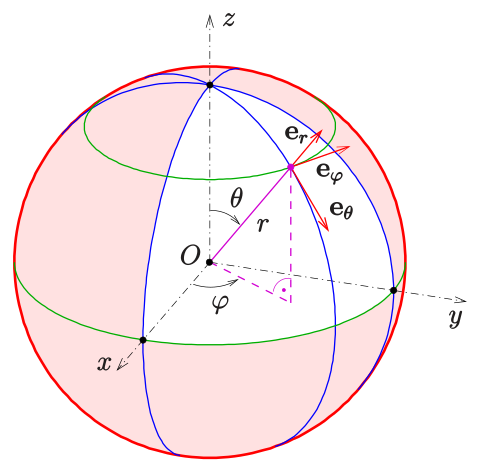
\includegraphics[width=0.5\textwidth]{figure/sphere.png}
            \caption{球坐标系的基底选择}
            \label{fig:spherecoordinate}
        \end{figure}
        
        我们需要将Laplace算符改写成球坐标系下的形式,因此我们要对算符进行坐标变换。根据示意图,我们可以直接写出直角坐标与球坐标间的变换关系:
        \begin{align}
            \begin{split}
                x=&rsin\theta cos\varphi\\
                y=&rsin\theta sin\varphi\\
                z=&rcos\theta
            \end{split}
        \end{align}
        
        代入Laplace算子中我们可以知道其在球坐标系下的形式\footnote{具体计算可以参考田光善的量子力学讲义Ch0}:
        \begin{equation}
            \nabla^2=\frac{1}{r^2}\frac{\partial}{\partial r}\Big(r^2\frac{\partial}{\partial  r}\Big)+\frac{1}{r^2\sin{\theta}}\frac{\partial}{\partial \theta}\Big(\sin{\theta}\frac{\partial}{\partial \theta}\Big)+\frac{1}{r^2\sin{\theta}}\frac{\partial^2}{\partial\varphi^2}
        \end{equation}
        
        代入本征方程\ref{equ6:stationaryequB}式,可以得到:
        \begin{equation}
            \frac{\hbar^2}{2m_e}\Big(\frac{1}{r^2}\frac{\partial}{\partial r}\Big(r^2\frac{\partial\psi}{\partial  r}\Big)+\frac{1}{r^2\sin{\theta}}\frac{\partial}{\partial \theta}\Big(\sin{\theta}\frac{\partial\psi}{\partial \theta}\Big)+\frac{1}{r^2\sin^2{\theta}}\frac{\partial^2\psi}{\partial\varphi^2}\Big)+V\psi =E\psi
        \end{equation}
        
        可以发现,由于$V=V(r)$,因此上述方程是可以分离变量的。令$\psi(r,\theta,\varphi)=R(r)Y(\theta,\varphi)$,可以得到:
        \begin{equation}
            \frac{\hbar^2}{2m_e}\Big(\frac{Y}{r^2}\frac{\partial }{\partial r}\Big(r^2\frac{\partial R}{\partial  r}\Big)+\frac{R}{r^2\sin{\theta}}\frac{\partial }{\partial \theta}\Big(\sin{\theta}\frac{\partial Y}{\partial \theta}\Big)+\frac{R}{r^2\sin^2{\theta}}\frac{\partial^2 Y}{\partial\varphi^2}\Big)+(V-E)RY=0
        \end{equation}
        
        等号两边同时除以RY,并且同时乘以$-\frac{2m_e}{\hbar^2}$,可得:
        \begin{equation}
            \Big\{\frac{1}{R}\frac{d}{dr}\Big(r^2\frac{dR}{dr}\Big)-\frac{2m_e}{\hbar^2}(V-E)\Big\}+\frac{1}{Y}\Big\{\frac{1}{\sin{\theta}}\frac{d}{d\theta}\Big(\sin{\theta}\frac{dY}{d\theta}\Big)+\frac{1}{\sin^2{\theta}}\frac{d^2Y}{d\varphi^2}\Big\}=0
        \end{equation}
        
        按照分离变量法的步骤,两个大括号相等当且仅当这两个大括号等于一个常数,我们令常数为$l(l+1)$\footnote{为什么常数的形式是$l(l+1)$将在后续内容中解释},则我们可以得到两个本征方程:
        
        \begin{align}
            \begin{split}
                \frac{1}{R}\frac{d}{dr}\Big(r^2\frac{dR}{dr}\Big)-\frac{2m_e}{\hbar^2}(V-E)=&l(l+1)\\
                \frac{1}{Y}\Big\{\frac{1}{\sin{\theta}}\frac{d}{d\theta}\Big(\sin{\theta}\frac{dY}{d\theta}\Big)+\frac{1}{\sin^2{\theta}}\frac{d^2Y}{d\varphi^2}\Big\}=&-l(l+1)
            \end{split}
        \end{align}
        \subsection{角动量方程的求解}
            本节我们考虑$Y(\theta,\varphi)$对应的本征方程:
            \begin{equation}
                \frac{1}{Y}\Big\{\frac{1}{\sin{\theta}}\frac{d}{d\theta}\Big(\sin{\theta}\frac{dY}{d\theta}\Big)+\frac{1}{\sin^2{\theta}}\frac{d^2Y}{d\varphi^2}\Big\}=-l(l+1)
            \end{equation}

            等号两边同时乘以$Y\sin^2{\theta}$可以得到:
            \begin{equation}
                \sin{\theta}\frac{d}{d\theta}\Big(\sin{\theta}\frac{dY}{d\theta}\Big)+\frac{d^2Y}{d\varphi^2}+l(l+1)\sin{\theta}Y=0
            \end{equation}
            
            我们发现该式同样能够分离变量:$Y(\theta,\varphi)=\Theta(\theta)\Phi(\varphi)$,代入可得:
            \begin{equation}
                \Phi\sin{\theta}\frac{d}{d\theta}\Big(\sin{\theta}\frac{d\Theta}{d\theta}\Big)+\Theta\frac{d^2\Phi}{d\varphi^2}+l(l+1)\sin{\theta}\Theta\Phi=0
            \end{equation}
            
            等号两边同时除以$\Theta\Phi$,可得:
            \begin{equation}
                \frac{\sin{\theta}}{\Theta}\frac{d}{d\theta}\Big(\sin{\theta}\frac{d\Theta}{d\theta}\Big)+l(l+1)\sin{\theta}+\frac{1}{\Phi}\frac{d^2\Phi}{d\varphi^2}=0
            \end{equation}
            
            自然我们可以得到两个本征方程,设此时的分离常数为$m^2$,那么:
            \begin{align}
                \begin{split}
                    \frac{\sin{\theta}}{\Theta}\frac{d}{d\theta}\Big(\sin{\theta}\frac{d\Theta}{d\theta}\Big)+&l(l+1)\sin{\theta}=m^2\\
                    \frac{1}{\Phi}\frac{d^2\Phi}{d\varphi^2}=-m^2
                \end{split}
            \end{align}
            
            先看$\Phi(\phi)$的方程,这是一个简单的微分方程,经过简单计算,我们可以得到通解为:
            \begin{equation}
                \Phi(\varphi)=Ae^{im\varphi}
            \end{equation}
            
            这里本来有两个解$e^{im\varphi},e^{-im\varphi}$的,但是由于$m$的取值既可以取正也可以取负,因此这两个解是线性相关的,只取一个就可以了。考虑边界条件,由于在球坐标的定义下,当$\varphi$转过$2\pi$角度时,粒子应该回到同一点,因此边界条件应该是周期条件:$\Phi(\varphi+2\pi)=\Phi(\varphi)$,因此:
            \begin{equation}
                e^{im\varphi}=e^{im(\varphi+2\pi)}\Rightarrow e^{2\pi im}=1,m=0,\pm 1,\dots
            \end{equation}
            
            归一化常数$A$可以通过$\Theta$的归一化可以求得:
            \begin{equation}
                \int_0^{2\pi}\Phi^*(\varphi)\Phi(\varphi)d\varphi=\int_0^{2\pi}A e^{im\varphi}\cdot Ae^{im\varphi}d\varphi=2\pi A^2=1
            \end{equation}
            
            于是可以得到:$A=\frac{1}{\sqrt{2\pi}}$,于是解的形式:
            \begin{equation}
                \Phi(\varphi)=\frac{1}{\sqrt{2\pi}}e^{im\varphi}
            \end{equation}
            
            下面讨论有关$\Theta(\theta)$的方程:
            \begin{equation}
                \frac{1}{\sin{\theta}}\frac{d}{d\theta}\Big(\sin{\theta}\frac{d\Theta}{d\theta}\Big)+\Big(l(l+1)-\frac {m^2}{\sin^2{\theta}}\Big)
            \end{equation}
            
            在附录B中我们介绍了Sturm-Liouville方程在Hilbert空间中具有重要意义。上式对比Sturm-Liouville方程的形式:
            \begin{equation}
                \frac{d}{dx}\Big(p(x)\frac{dy}{dx})+(q(x)+\lambda)x=0
            \end{equation}
            
            我们可以发现形式已经大致相似了,唯一有问题的地方就是三角函数,于是我们作坐标变换:$z=\cos{\theta},z\in \mathbb{R}[-1,1];P(z)=\Theta(\theta)$,则:
            \begin{align}
                \begin{split}
                    \frac{d\Theta}{d\theta}=&\frac{dP}{dz}\cdot \frac{dz}{\theta}=\frac{dP}{dz}\sin{\theta}\\
                    \sin^2{\theta}=&1-z^2
                \end{split}
            \end{align}
            
            代入可得:
            \begin{equation}
                \frac{d}{dz}\Big((1-z^2)\frac{dP}{dz}\Big)+\Big(l(l+1)-\frac{m^2}{1-z^2}\Big)P=0
            \end{equation}
            %补充Sturm-Liouville方程具有的性质
        \subsection{径向方程的求解}
        
        现在考虑径向方程:
        \begin{equation}
            \frac{1}{R}\frac{d}{dr}\Big(r^2\frac{dR}{dr}\Big)-\frac{2m_e}{\hbar^2}(V-E)=l(l+1)
        \end{equation}
        
        我们同样考虑将其转换成Sturm-Liouville方程的形式。等号两边同乘$\frac{R}{r^2}$,可以得到:
        \begin{equation}
            \frac{1}{r^2}\frac{d}{dr}\Big(r^2\frac{dR}{dr}\Big)-\Big[\frac{2m}{\hbar^2}\Big(\frac{Ze^2}{r}-E\Big)+\frac{l(l+1)}{r^2}\Big]R=0
        \end{equation}
        
        由于电子和核子之间的相互作用是既有吸引也有排斥的,因此我们需要对E的正负号进行分类讨论。如果E<0,此时电子和核子之间以吸引力为主,较为稳定,不会发生电离;当E>0时,此时氢原子会发生电离,此时电子会遵循自由粒子的运动情况。在一般情况下,我们还是研究稳定的体系,因此在这里E<0。求解是类似的思路,首先我们希望通过去量纲化得到更为普遍的方程形式。